\chapter[Quasi-analytic classes of functions...]{Quasi-analytic classes of functions
  (Quasi-analyticity\\ $D$ and $I$ )}\label{chap19}%lect 19 

\section{Quasi-analyticity and mean periodicity}\label{chap19:sec1} % sec 1

We\pageoriginale shall see presently that problems of quasi-analyticity appear in a
natural way as problems on mean periodic functions. 
\begin{enumerate} [1.]
\item Consider the following problem. Given a set $E$ consider the
 closed span $\tau_E (f)$ of translates $f_y, y \in E$, of $f$. Find
 the conditions on $f$ in order that $\tau_E (f) = \tau (f)$. In
 other words, the problem, in a restricted sense, is to find a
 relation between $E$ and the spectrum $S(f)$ in order that $\tau_E
 (f) = \tau (f)$. 
\item On the other hand, the above problem suggests the following
 one. Let $f$ be a $C^\infty$- function and let $\delta (f)$ be the
 closed span of the derivatives of $f$. (When $E$ is not a discrete
 set, $\delta (f)$ is a subset of $\tau_E (f))$. Find conditions
 about $f$ so that $\delta (f) = \tau (f)$. Here we require a
 condition involving a class of $C^\infty$- functions, i.e. a
 condition on the class and the spectrum $S(f)$, for example
 conditions of the type $\{K \{M_n\}, S (f) \}, f \in K \big \{M_n
 \big \}$. 
\end{enumerate}

\begin{defi*} %def
 The class $ K \big \{M_n \big \}$ is defined to be the class of
 $C^\infty$- functions $f$ such that on every interval $I$, $\big |
 f^{(n)} \big |_I < K_I M_n$, $(n = 0, 1, \ldots ),$ where $ \big
 \{M_n \big \}$ is a given sequence and $K_I$ a constant depending on
 $I$ and $f$. $C \big \{M_n \big \}$ is defined as a class of
 $C^\infty$- functions which satisfy the relation $\big | f^{(n)}
 \big | < KM_n$ on the real line, $K$ depending only on $f$. 
\end{defi*}

The above two problems are closely related to quasi-analyticity.

\begin{enumerate}
\item In\pageoriginale order that $\tau_E (f) = \tau (f)$ it is necessary and
 sufficient (condition of Riesz) that every measure $d \mu$
 orthogonal to $\tau_E (f)$ be orthogonal to $\tau (f)$. Or again,
 $g(y) = \int f (x + y)d \mu(-x) = 0$ for every $y \in E
 \Rightarrow g \equiv 0$. As $f \in \mathscr{C}_\Lambda$ implies $g
 \in \mathscr{C}_\Lambda$, we 
 have an answer to this problem if we have a relation $R \{E, \Lambda
 \}$ between $E$ and $\Lambda$ such that $\{ g \in
 \mathscr{C}_\Lambda, g (y) = 0, y \in E \} \Rightarrow g \equiv
 0$. This is nothing but a problem of uniqueness. We will be mainly
 interested in the case when $E$ is an interval. 

 \begin{defi*}%defi 0
 A class of functions is called an I-quasi-analytic class if each
 function of the class is defined by its values on $I, I$ being an
 interval. 
 \end{defi*}
\item By the condition of Riesz, denoting by
 $$
 \displaylines{\hfill 
 g(y) = \inf f (x+y) d \mu (-x),\hfill \cr
 \text{we have}\hfill \delta (f) =
 \tau (f) \Leftrightarrow \big [ g^{(n)} (0) = 0~ \forall n
  \Rightarrow g \equiv 0 \big].\hfill } 
 $$
 When $f$ has spectrum $\Lambda, g \in \mathscr{C}_\Lambda$. Moreover
 if $f \in K \{ M_n \}$ then $g \in K \{M_n\}$ so that $g \in K \{M_n\}
 \cap \mathscr{C}_\Lambda$. Thus we have an answer to this problem if we
 have a relation $\{\{ M_n\}, \Lambda \}$ such that $\{g \in K \{M_n\}
 \cap \mathscr{C}_\Lambda, g^{(n)} (0) = 0 \forall n \} \Rightarrow g
 \equiv 0$. The same is true in replacing $K\{M_n\}$ by $C \{N_n\}$.  
 \begin{defi*}%defi 0
  A class of $C^\infty$ - functions is defined as a D-quasi-analytic
  class if the only function $g$ of the class all of whose derivatives
  vanish at the origin is the zero function. 
 \end{defi*}
\end{enumerate}

In Lecture 5 \S \ref{chap5:sec2}, we proved a result equivalent to the following:
$\mathscr{C}_\Lambda$ is an I-quasi-analytic class if $| I | >$
mean-period related to $\Lambda$. We give here a far stronger result. 

\begin{theorem*}
 Let\pageoriginale $\Lambda $ be a sequence of complex numbers such that
 $\mathscr{C}_\Lambda \neq \mathscr{C}$, and $\Lambda^*$ and
 $\Lambda^-$ the parts of $\Lambda$ respectively to the right and to
 the left of the imaginary axis. $\mathscr{C}_\Lambda$ is a quasi -
 analytic class whenever
 $$
 | I| > 2 \pi D_{\min} (\Lambda^+) \text { or } | I | > 2 \pi
 D_{\min} (\Lambda^-). 
 $$
\end{theorem*}

\begin{proof}
 We use the notations of Lecture $4$. $f \in \mathscr{C}_\Lambda, f *
 d \mu = 0, f^{-1} * d \mu = g , ~ F(w) =
 \dfrac{G(w)}{M(w)}, S (f)=$ spectrum of $f$. Denoting by $\sum (d
 \mu) $ and $ \sum (g) $ the null-sets of $M(w)$ and $G(w)$, we have
 $S(f) = \sum (d \mu) - \sum (g) \cap \sum (d \mu)$. Let $L_\mu$ and
 $L_g$ be the lengths of the segments of supports of $d \mu$ and
 $g$. According to Levinson's theorem, $L = 2 \pi $ density $\sum \pm
 (d \mu) ~ (\sum \pm$ is the part of $\sum $ to the right
 (respectively to the left) of the imaginary axis). Now we use the
 result that if $S_1$ and $S_2$ are disjoint sequences, and $S = S_1
 \cup S_2$ has a density, density $S = D_{\max} S_1 + 
 D_{\min} S_2$. Thus $L = 2 \pi D_{\min} S^\pm (f) + 2 \pi D_{\max}
 (S^\pm (g) \cap S^\pm (d \mu)); L_\mu \le 2 \pi D_{\min} S^\pm (f) +
 L_g$. If $f = 0$ on $(-1, 0)$, then $L_g \le L- 1$. Hence 
 $$
 D_{\min} S^+ (f) \ge (L_\mu - L_g)/ 2 \pi \ge 1/2 \pi.
 $$

 So if $1>2 \pi D_{\min} S^+ (f) $ or $ 1 > 2 \pi D_{\min} S^- (f), f
 \equiv 0$. As a translation of $f$ does not change $S(f)$, the theorem
 is proved. 
\end{proof}

The above theorem is stated in Levinson (Levinson, chap. $II$), when
$\Lambda$ is a sequence of integers, i.e. $f$ is a periodic function;
then the proof does not require the Carleman transform of $f$. 

\section{Theorem of Denjoy-Carleman}\label{chap19:sec2}%sect 2

We first study D-quasi-analytic classes in which no condition on
$\Lambda$ is involved. We shall prove a classical theorem of
Denjoy-Carleman about D-quasi-analytic classes. It is a local property
and so can be stated for an interval. 

\begin{defi*}%defi 0
 Let\pageoriginale $C_I \{M_n\}$ be $\in $ class of $C^\infty$- functions
 satisfying the conditions $\big | f^{(n)} (x) \big | < K M_n$ on an
 interval $I, 0 \in I, K$ depending only on $f$. We say that it is a
 quasi-analytic class if $f^{(n)} (0) = 0$ for every $n \Rightarrow f
 \equiv 0$. 

 Given a sequence $\{M_n\}$ let $\{M^C_n\}$ be the largest sequence
 which satisfies $M^c_n \le M_n$ and $M^c_{n+1}/ M^c_n \nearrow$. 

 \noindent
 \textbf{Theorem of Denjoy-Carleman}. $C_I \{M_n\}$ is a quasi-
 analytic class $\Leftrightarrow \sum\limits_1^\infty
 \dfrac{M^c_n}{M^c_{n+1}} = \infty$. 
 
 A variant of this theorem (stated by Denjoy without proof) is that
 $C_I \{M_n\}$ is a quasi-analytic class $\Leftrightarrow
 \sum\limits_1^\infty \dfrac{1}{(M^c_n)^1/n} = \infty$. The
 equivalence of these two follows from the inequality: 
 $$
 \sum \in_n < \sum (\in_1 \cdots \in_n)^{1 /
 n } < e \sum \in_n \text { for } \in_n \searrow
 0. 
 $$
 (Cf. Hary-Littlewood-Polya: Inequalities, or $S$. Mandelbrojt $2$).
\end{defi*}

\noindent
\textbf{Interpretation of } $M_n$. Consider in the plane the points
($n, \log M_n)$ and construct the polygon of Newton on these
points. It is a convex curve $m(u)$. The ordinate at $n$ intersecting
this curve gives $\log M^c_n$. The sequence $\{\log M^c_n \}$ is
called the convex regularized sequence corresponding to $\{\log
M_n\}$. (Mandelbrojt $2$). 

\begin{proofofthm*}%theo 0
 We can suppose $I \supset \big [ 0, 1\big], K = M_o = 1$ and $M_n =
 M^c_n$. Consider $\varphi (x) = f(x) f(1-x)$ in $0 \le x \le 1$ and
 $\varphi (x) = 0$ elsewhere. Since $\log M_n$ is convex, $M_n$ is
 the $\max \limits_{i \le n} (M_i M_{n - i})$. Thus we have the
 following majorization for $\varphi^{(n)} (x)$: 
 $$
 \big | \varphi^{(n)} (x) \big | \le M M_n + (^n_1) M_1 M_{n-1} +
 \cdots + M_n M_o \le 2^n M_n 
 $$
 and $\varphi$ is null, with all its derivatives, at the
 origin. Consider $\Phi (w) = \tau (\varphi) = \int^1_0 \varphi (x)
 e^{-ixw} dw$.\pageoriginale Integrating by parts, we have 
 $$
 \Phi (w) = \int^1_o
 \varphi^{(p)}(x) \dfrac{e^{- ixw}}{(iw)^p} dx \quad
 \text{and}\quad \big | \Phi (w) \big | < 2^p M_p \big / | w | P.
 $$ 
\end{proofofthm*}

Now we introduce the function $T(r) = \sup\limits_{p} r^P/M_p$. Then
$\big | \Phi (w) \big | < \dfrac{1}{T (r/2)}$. We apply Carleman's
formula for $\Phi (w)$ in the upper or lower half plane and get
$\int^R \dfrac{\log \{ \Phi (u) \Phi (-u)\}}{u^2} du$ cannot tend to
$- \infty$. Since $\big | \Phi (w) \big | < \dfrac{1}{T(r/2)'}$, we have
$\int^\infty \dfrac{\log T(r)}{r^2} dr < \infty$. Therefore
$\int^\infty \dfrac{\log T(r)}{r^2}$ $dr = \infty$ implies
quasi-analyticity (Ostrowski's form). 

We have $\log T(e^\sigma) = t (\sigma) = \max\limits_{n} (n \sigma -
\log M_n) = \max\limits_{u} (\sigma u - m (u))$. Moreover the relation
between $t(\sigma)$ and $m(u) $ is reciprocal. Indeed\break $m(u
) = \max (u \sigma - t(\sigma)) $. Also the derivatives $t' (\sigma)$
and $m'(u)$ are inverse functions in a sense made precise by the
graph. First we suppose $m(u) \to \infty$ when $u \to \infty$. Now 
$$
\int^X e^{- \sigma} t (\sigma) d \sigma = - e^X t(X) + \int^X e^{-
 \sigma} t' (\sigma) d \sigma 
$$ 
\begin{figure}[H]
 \centerline{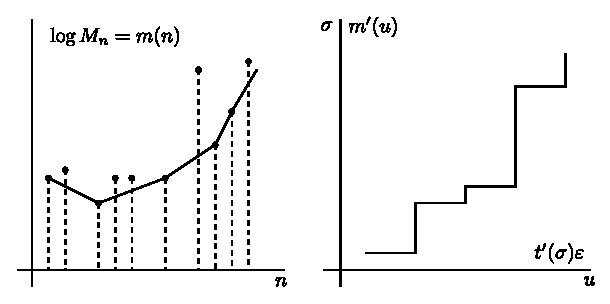
\includegraphics{vol15-figures/fig15-21.eps}}
\end{figure}

Thus\pageoriginale we have $\int^\infty e^{- \sigma} t (\sigma) d \sigma = \infty
\Leftrightarrow \int^\infty e^{- \sigma} t' (\sigma) d \sigma =
\infty$. 
 
Since $\sigma = m' (u)$ and $u = t' (\sigma)$, we have the following relations:
\begin{gather*}
 \int^T e^{-m'(u)} udm' (u) = - e^{-m' (T)} T+ \int^T_ \infty e^{- m' (u)} du\\
 \int^\infty e^{- \sigma} t' (\sigma) d \sigma \quad = \infty
 \Leftrightarrow \int^\infty e^{- m' (u)} du = \infty. 
\end{gather*}

Between $n \le u \le n + 1, m'(u) = \log M_{n+1} - \log M_n$ and $-
m'(u) = \log \dfrac{M_n}{M_{n+1}}$. 
\begin{align*}
 \int^\infty e^{-m' (u)} du &= \infty \Leftrightarrow \sum
 \frac{M_n}{M_{n+1}}= \infty\\ 
 \int^\infty \frac{\log T(r)}{r^2} dr & = \infty \Leftrightarrow
 \int^\infty e^{- \sigma} t (\sigma) d \sigma = \infty. 
\end{align*}

Thus, finally we have the relation
$$
\int^\infty \frac{\log T(r)}{r^2} dr = \infty \Leftrightarrow
\int^\infty \frac{M^C_n}{M^{C+1}_{n+1}} = \infty. 
$$

This relation still holds when $m'(u)$ is bounded.

We have proved that if $\sum M^C_n / M^C_{n+1} = \infty, C_I \{M_n\} $
is a quasi-analytic class. Suppose $\sum M^C_n / M^C_{n+1} <
\infty$. Then we construct a $C^\infty$- function with compact support
which is $ \nequiv 0$ and which satisfies the conditions $\big | f^{(n)}
\big | < M^c_n$ and $f^{(n)} (0) = 0$ for every $n$. To construct $f$
it is convenient to construct its transform. 

Take $F(w) = \left(\dfrac{\sin \in w}{\in w}\right)^2
\prod\limits_{1}^\infty \dfrac{\sin \alpha_j w}{\alpha_j w}$. It is an
entire function of exponential type if $\sum \alpha_j < \infty,
\alpha_j > 0$. We can majorise $\big | \dfrac{\sin \alpha_j
 u}{\alpha_j u} \big | $ by $1$ for $j \ge N$ and we have $\big |
F(u) \big | < \left(\dfrac{\sin \in u}{\in u}\right)^2
\prod\limits_{1}^N \dfrac{1}{| \alpha_j u |}$. 

We write $F (w) = \mathscr{C}(f), f(x) = \dfrac{1}{2 \pi}
\int^\infty_{- \infty} F(u) e^{iux} du$, since $F(u)$ is rapidly
decreasing. Also we have the following relations: 
\begin{align*}
 f^{(n)} (x) & = \frac{1}{2 \pi} \int^\infty_{- \infty} F(u) (iu)^n e^{ixu} du\\
 \big | f^{(n)} (x) \big | & < (\alpha_1 \cdots \alpha_n)^{-1}
 \int^\infty_{- \infty} \left(\dfrac{\sin \in u}{\in u}\right)^2
 du. 
\end{align*}

We take $M^c_n = (\alpha_1 \cdots \alpha_n)^{-1}$, i.e. $\alpha_n =
M^C_n/M^{C-\infty}_{n+1}$. 

Thus our construction is complete.
